\documentclass{article}

% if you need to pass options to natbib, use, e.g.:
%     \PassOptionsToPackage{numbers, compress}{natbib}
% before loading neurips_2019

% ready for submission
% \usepackage{neurips_2019}

% to compile a preprint version, e.g., for submission to arXiv, add add the
% [preprint] option:
\usepackage[preprint]{neurips_2019}

% to compile a camera-ready version, add the [final] option, e.g.:
%\usepackage[]{neurips_2019}

% to avoid loading the natbib package, add option nonatbib:
%     \usepackage[nonatbib]{neurips_2019}

\usepackage[utf8]{inputenc} % allow utf-8 input
\usepackage[T1]{fontenc}    % use 8-bit T1 fonts
\usepackage{hyperref}       % hyperlinks
\usepackage{url}            % simple URL typesetting
\usepackage{booktabs}       % professional-quality tables
\usepackage{amsfonts}       % blackboard math symbols
\usepackage{amssymb}        % lessapprox
\usepackage{amsmath}        % cases
\usepackage{nicefrac}       % compact symbols for 1/2, etc.
\usepackage{microtype}      % microtypography

\usepackage[pdftex]{graphicx}

\title{Empirical quantification of privacy loss with examples relevant to the 2020 US Census}

% The \author macro works with any number of authors. There are two commands
% used to separate the names and addresses of multiple authors: \And and \AND.
%
% Using \And between authors leaves it to LaTeX to determine where to break the
% lines. Using \AND forces a line break at that point. So, if LaTeX puts 3 of 4
% authors names on the first line, and the last on the second line, try using
% \AND instead of \And before the third author name.

\author{%
  Abraham D.~Flaxman \\
  Department of Health Metrics Sciences\\
  University of Washington\\
  Seattle, WA, USA \\
  \texttt{abie@uw.edu} \\
  % examples of more authors
  % \AND
  % Coauthor \\
  % Affiliation \\
  % Address \\
  % \texttt{email} \\
  % \And
  % Coauthor \\
  % Affiliation \\
  % Address \\
  % \texttt{email} \\
  % \And
  % Coauthor \\
  % Affiliation \\
  % Address \\
  % \texttt{email} \\
}

\begin{document}

\maketitle

\begin{abstract}
  The 2020 US Census will use differential privacy for disclosure avoidance, employing a new algorithm called TopDown to guarantee privacy loss of at most $\epsilon$.  However, it is possible that there is some slack in the bound (which is proven using the sequential composition theorem), and in practice, the privacy loss will be substantially less than $\epsilon$.
  
  In this paper, I develop an empirical measure of privacy loss, and apply it to three  example algorithms, inspired by some aspects of TopDown, to better understand how the empirical privacy loss might compare to the theoretical guarantee.
  
  My results suggest that (1) it is possible to quantify privacy loss empirically in a reasonable amount of time, at least for counting algorithms like TopDown; and (2) it is likely that the empirical privacy loss of hierarchical counting algorithms like TopDown is substantially lower than the privacy bound derived from the serial composition theorem.
\end{abstract}

\section{Introduction}

The 2020 US Census will use a new approach to disclosure avoidance to protect respondents' data.\cite{abowd2018disclosure} This approach relies on $\epsilon$-Differential Privacy (DP), a mathematical definition of privacy that has been developed over the last decade and a half in the theoretical computer science and cryptography communities. $\epsilon$-DP is not an algorithm, it is a property that an algorithm might satisfy.\cite{dwork2014algorithmic}

The Census Bureau has developed their algorithm, TopDown, to be $\epsilon$-DP with low error, by applying a geometric mechanism repeatedly, at multiple levels of a geographic hierarchy, and using constrained optimization to combine the noisy measurements and ensure consistency at each level.\cite{abowd2019census}  Although the sequential composition theorem of DP ensures that the total privacy loss of TopDown is at most $\epsilon$, it is possible that this inequality is not tight.

To better understand how much privacy will be delivered by TopDown, I investigated the privacy loss of an idealized top-down algorithm and compared it to other simple counting algorithms.  My estimates of empirical privacy loss relied on a nonparametric method from machine learning (kernel density estimation), and offer directions for future application of sophisticated machine learning tools.

\section{Methods}
\label{methods}

An algorithm $\mathcal{A}$ is $\epsilon$-DP if for each possible output
$\mathcal{P}$, for any pair of datasets $D$ and $D'$ that are the same
everywhere except for on one person's data,
$$
\Pr\left[\mathcal{A}(D) = \mathcal{P}\right]
\leq \exp\left(\epsilon\right)
\Pr\left[\mathcal{A}(D') = \mathcal{P}\right].
$$

At a high level, the TopDown algorithm produces differentially private counts of people in multiple
demographic groups for hierarchically nested areal units (e.g. census tracts in counties in states).
To do this, it repeats two steps at multiple levels of a geographic
hierarchy (from the top down, hence the name). First,
it adds noise from an appropriate probability distribution
to the exact data counts to produce a set of noisy counts. Then, it adjusts
these counts to
be close as possible to the noisy counts, subject to the constraints
that all counts be non-negative and consistent with each other and the higher levels
of the hierarchy, and satisfy certain invariants and other inequalities.  These
two steps are performed for each geographic level, from the coarsest
to the finest.  Each level is designed to exhaust a privacy budget of $\epsilon_i$,
so, by the sequential composition theorem, 
the entire algorithm achieves $\epsilon$-DP for $\epsilon=\sum_{i=1}^6
\epsilon_i$.

\subsection{Simulation strategy for generating synthetic individuals to count}
To better understand how DP counting algorithms perform, I generated a synthetic population of $N$ individuals, each with a location specified by $J$ hierarchically nested levels, designed to have an average of $\mu$ individuals per location.
I represented this database as matrix $D$ with $N$ rows and $J$ columns, where row $D_i$ represented the areal unit inhabited by individual $i$.
To assign this areal unit, for each individual $i$, for each level of the spatial hierarchy $j$, I sampled the location uniformly at random, $D_{ij} \sim_{\mathcal{U}} \{0, 1, \ldots, C-1\}$, where $C = \left\lfloor \left(N/\mu\right)^{1/J} \right\rfloor$ is the number of children for every areal unit in the spatial hierarchy before level $J$ (e.g. the number of census tracts in each county is $C$ in my simulation).

To find the exact total count (TC) for each location at any level of the spatial hierarchy, I grouped the database $D$ by spatial area and counted how many individuals were in each areal unit:
$$
\mathrm{TC}_{j_1, j_2, \ldots, j_{J'}} = \sum_i \mathbf{1}\left[
D_{i,1} = j_1 \wedge 
D_{i,2} = j_2 \wedge 
\ldots
D_{i,J'} = j_{J'}
\right].
$$

\subsection{Three DP algorithms for counting total individuals}
\emph{Geometric Noise:} To generate $\epsilon$-DP counts from exact counts, I used the geometric mechanism to add noise to the exact counts for the most fine-grained areal units in the spatial hierarchy (abbreviated GDPC for geometric DP count):
$$
\mathrm{GDPC}_{j_1, j_2, \ldots, j_{J}} = \mathrm{TC}_{j_1, j_2, \ldots, j_{J}} + X_{j_1, j_2, \ldots, j_{J}},
$$
where $X_{j_1, j_2, \ldots, j_{J}} \sim G(\epsilon)$ is drawn from a two-tailed geometric distribution with parameter $\epsilon$, defined by the following equation
$$\Pr[G(z)=k] = \frac{(1 - \exp(-z))\exp(-z|k|)}{1 + \exp(-z)}.$$
The output of this algorithm is the list of $
\mathrm{GDPC}_{j_1, j_2, \ldots, j_{J}}$ values for all tuples $(j_1, j_2, \ldots, j_{J})$.

\emph{Raked Geometric Noise:} To capture a key element of the TopDown algorithm, I also generated $\epsilon$-DP counts from exact counts hierarchically, by ``raking'' the noisy counts at each level to sum to the noisy count from the level above.

To be precise, for level $J'$ of the spatial hierarchy, I first calculated noisy counts analogous to $\mathrm{GDPC}$, but using only a $1/(J+1)$ portion of the total privacy budget:
$$
\mathrm{NoisyC}_{j_1, j_2, \ldots, j_{J'}} = \mathrm{TC}_{j_1, j_2, \ldots, j_{J'}} + X_{j_1, j_2, \ldots, j_{J'}},
$$
where $X_{j_1, j_2, \ldots, j_{J'}} \sim G(\epsilon/(J+1))$.
I then obtained the raked DP counts (RDPC) by scaling the noisy counts for the children of each areal unit at level $J'-1$ of the spatial hierarchy, so that the sum of raked counts at level $J'$ was equal to the raked DP count for their parent:
$$
\mathrm{RDPC}_{j_1, j_2, \ldots, j_{J'}} = 
\mathrm{NoisyC}_{j_1, j_2, \ldots, j_{J'}}\cdot
\left(\frac
{\mathrm{RDPC}_{j_1,j_2,\ldots, j_{J'-1}}}
{\sum_{j'=1}^C \mathrm{NoisyC}_{j_1, j_2, \ldots, j_{J'-1}, j'}}
\right)
$$

To start this process, I defined the RDPC for $J' = 0$ as
$\mathrm{RDPC}_{\{\}} = N + X_{\{\}}$, where $X_{\{\}} \sim G(\epsilon/(J+1))$.

The output of this algorithm is the list of $
\mathrm{RDPC}_{j_1, j_2, \ldots, j_{J'}}$ values for all tuples $(j_1, j_2, \ldots, j_{J'})$ for all $J' \leq J$.

\emph{Averaged Geometric Noise:} As a comparison, I considered a algorithm which produced an average multiple noisy measurements that is provably $\epsilon$-DP.  As with the raked approach, I split the total privacy budget equally into $P$ parts, but I then used each portion to run the geometric mechanism with the smaller epsilon, and obtained the Average-of-Geometrics DP counts (ADPC) from their arithmetic mean:
$$
\mathrm{ADPC}_{j_1,j_2,\ldots, j_{J}} =
\frac{1}{P}\sum_{p=1}^P
\mathrm{GDPC}_{j_1, j_2, \ldots, j_{J}}^p,
$$
where $\mathrm{GDPC}_{j_1, j_2, \ldots, j_{J}}^p$ is the output of an independent replicate of the GDPC algorithm with privacy budget $\epsilon/P$.

\subsection{Empirical estimation of privacy loss}
Differentially private algorithms are often engineered to achieve a guaranteed maximum level of privacy loss (for example GDPC, RDPC, and ADPC are all $\epsilon$-DP).  However, in complex algorithms like TopDown or RDPC, this bound on the privacy loss might have room for improvement.  I tested two approaches to empirically measuring privacy loss, to see how the theoretical bounds of $\epsilon$ from the algorithms above compare to the privacy loss demonstrable in practice.

The most direct way to empirically investigate the privacy loss of an algorithm $\mathcal{A}$ like those from the previous section is to search for databases $D$ and $D'$ that differ on a single row and an event $E$ that can serve as a witness to the gap between $\Pr[\mathcal{A}(D) \in E]$ and $\Pr[\mathcal{A}(D') \in E]$.  Estimating the ratio of these probabilities is straightforward, but computationally intensive, and searching the space of near-databases and events is also difficult to do in general.  This approach has been developed in prior work by Ding et al (2019).\cite{ding2018detecting}  In the case of count queries with the $D$ defined in the previous section, the search simplifies substantially.  The symmetric nature of the database means we can focus on changing the first row, without loss of generality, and the discrete nature of the output means we can restrict our attention entirely to events $E$ of the form $\left\{\mathrm{error}_{j_1, j_2, \ldots, j_{J}}
= k\right\}$ or $\left\{\mathrm{error}_{j_1, j_2, \ldots, j_{J}} \geq k\right\}$ where $\mathrm{error}_{j_1, j_2, \ldots, j_{J}} = \mathcal{A}(D)_{j_1, j_2, \ldots, j_{J'}}
- \mathrm{TC}_{j_1, j_2, \ldots, j_{J'}}$, where $k$ is any integer.

\emph{Direct estimate:} I ran GDPC, RDPC, and ADPC 500 times with a single synthetic database $D$, generated as described above, and 500 more times with a perturbed database $D'$, created by changing the areal unit of a single individual (moving someone from area $0$ to area $1001$, where these areas were chosen arbitrarily). From these repeated realizations of the randomized algorithm, I estimated the probability of the count for areal unit $0$ being $k$ away from the exact total count for this area.  For any $k$, the log of the ratio of these probabilities constitutes a (noisy) lower bound on $\epsilon$, and the maximum over these log-ratios could be used as an empirical estimate of the privacy loss.

% With only 100 replicates of the results of the original and perturbed counts, however, these directly estimated log-ratios are too noisy to provide an interpretable bound.  To address this, I used Gaussian kernel density estimation, to estimate the probability of a residual of $k$ for the original and perturbed databases, $\tilde{p}_D(k)$ and $\tilde{p}_{D'}(k)$.  I experimented with a range of bandwidth parameters for the Gaussian, and used $\log\left( \tilde{p}_D(k) / \tilde{p}_{D'}(k)\right)$ as a less-noisy direct estimate of the empirical privacy loss.

\emph{Less-obvious estimate:} Because of the special structure of count queries, there is a way to avoid re-running the DP algorithm repeatedly.  This can be particularly useful for assessing the empirical privacy loss of complex algorithms like TopDown. If the difference between the DP count and the exact count was identically distributed for all areal units, then instead of focusing on only the areal units containing the individual who's changed, we could use the residuals for all areal units to estimate the probability of the event we are after:
$$\Pr\left[\mathrm{error}_{j_1, j_2, \ldots, j_{J}}^D
= k\right]
\approx
\bigg(\sum_{j_1'=1}^C\sum_{j_2'=1}^C\cdots\sum_{j_J' = 1}^C \mathbf{1}\left[\left\{\mathrm{error}_{j_1', j_2', \ldots, j_{J}'}^D
= k\right\}\right]\bigg)\bigg/C^J =: \hat{p}_k,
$$
and $$\mathrm{error}_{j_1, j_2, \ldots, j_{J}}^D = \left(\mathcal{A}(D)_{j_1, j_2, \ldots, j_{J'}}
- \mathrm{TC}_{j_1, j_2, \ldots, j_{J'}}\right),$$
where $\mathcal{A}(D)$ is the vector of DP counts returned by the GDPC, RDPC, or ADPC algorithm.

We can make this estimate with more precision than the direct estimate, using substantially less computation.

It is also possible to make an estimate of the probability $D'$ yields error of $k$ without repeatedly running the DP algorithm.  This relies on the observation that, for count queries, a change to a single row of data can change the exact count by at most one for any areal unit.  Therefore
$$
\Pr\left[\mathrm{error}_{j_1, j_2, \ldots, j_{J}}^{D'}
= k\right]
\gtrapprox
\begin{cases}
\Pr\left[\mathrm{error}_{j_1, j_2, \ldots, j_{J}}^{D}
= k+1\right], \qquad \text{ if } k \geq 0;\\[.1in]
\Pr\left[\mathrm{error}_{j_1, j_2, \ldots, j_{J}}^{D}
= k-1\right], \qquad \text{ if } k \leq 0;
\end{cases}
$$
which we can also approximate by examining the residuals for all areal units:
$$\Pr\left[\mathrm{error}_{j_1, j_2, \ldots, j_{J}}^{D'}
= k\right]
\gtrapprox 
\bigg(\sum_{j_1'=1}^C\sum_{j_2'=1}^C\cdots\sum_{j_J' = 1}^C \mathbf{1}\left[\left\{\mathrm{error}_{j_1', j_2', \ldots, j_{J}'}^D
= k\pm 1\right\}\right]\bigg)\bigg/C^J.
$$
With these estimate in mind, I ran GDPC and RDPC for a range of databases $D$, with multiple values of $N$, $J$, $\mu$, and $\epsilon$ and calculated $\log \hat{p}_k / \hat{p}_{k-1}$ for all $|k| \leq K$. I used the maximum log-ratio as an empirical comparator with the theoretical privacy loss $\epsilon$.  I also searched for the appropriate value of $K$ to bound the range of residuals, which I parameterized by selecting a residual percentile and scaling factor (e.g. take $K$ to be $1.5$ times the $95$-th percentile of the residuals).

As with the direct estimates, I found that the stochastic noise in $\hat{p}_k$ led to undesirable fluctuations in the empirical privacy loss bounds, and to address this, I used Gaussian kernel density estimates to smooth the approximations of $\hat{p}(k)$ as a function of $k$.  I experimented with a range of bandwidth parameters for the Gaussian, and used $\log \hat{p}(k) / \hat{p}(k+1)$ to create a less noisy estimate of the empirical privacy loss.

\section{Results}
\label{results}

My direct estimate of privacy loss took 2 hours of compute time to produce 500 samples, but was too noisy to be interpretable.
%KDE smoothing was also unsuccessful in reducing the noise (in the time available in my rush to the submission deadline).
By uses a comparison of $\left\{\mathcal{A}(D)_{j_1, j_2, \ldots, j_{J'}}
- \mathrm{TC}_{j_1, j_2, \ldots, j_{J'}}
\geq k\right\}$ (instead of equal to $k$), I did obtain results visually consistent with the proven DP bound of $\epsilon$.

My less-obvious estimate of privacy loss took 20 seconds of compute time even though I ran it for a range of $\epsilon$ values.  It produced bounds on privacy loss showing that geometric noise empirical privacy loss matching its theoretical bound, averaged geometric noise (with $P=4$) has empirical privacy loss roughly half of the theoretical bound, and raked geometric noise (with $J=3$) has empirical privacy loss roughly one quarter of the theoretical bound. (Figure 1)

\begin{figure}[h]
  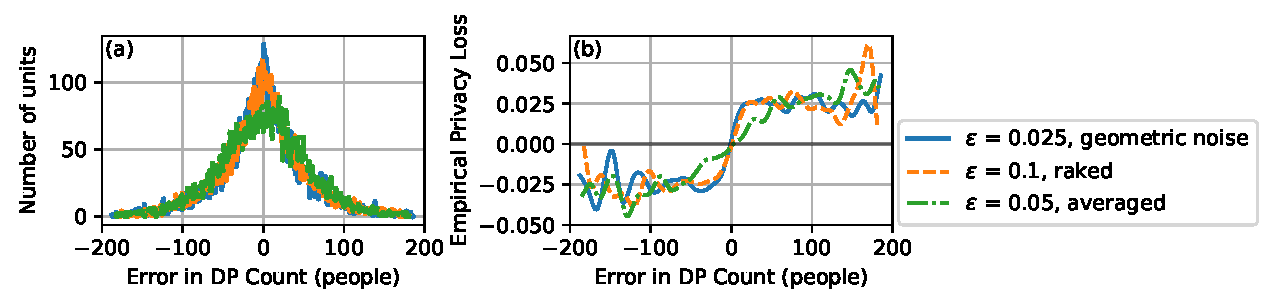
\includegraphics[width=\linewidth]{fig.pdf}
 \caption{Panel (a) shows the distribution of residuals (DP - Exact) for
GDPC, RDPC, and ADPC, each with an $\epsilon$ selected to have empirical privacy loss of $0.025$; and panel (b) shows the ``less-obvious'' estimate of empirical privacy
loss, smoothing with a kernel of bandwidth
$0.15$. This shows that for GDPC, the empirical privacy loss is equal to the budget of $0.025$, which for ADPC is it half of the budget of $0.05$ and for RDPC is is one quarter of the budget of $0.1$.}
\end{figure}

\section{Discussion and Conclusion}

This work is preliminary and certainly not without limitations.  My biggest concern with the general approach to empirically measuring privacy loss is that I could have missed something; if there is some alternative event $E$ which witnesses correlation introduced by the counting algorithm, this could prove there is greater privacy loss than either of the methods I described above would discover.  On the other hand, this work provides some evidence that the theoretical bounds produced by the sequential composition theorem are not always tight, and gives a way to estimate how much more private an algorithm like TopDown may be in practice.


\bibliographystyle{plain} % We choose the "plain" reference style
\bibliography{references} % Entries are in the "references.bib" file

Source code to reproduce the methods and results described in this paper can be found at \url{https://github.com/aflaxman/eqpl_w_examples}.

I would like to thank Andrew Dolgert for calling my attention to the similarities between the TopDown algorithm and raking.
\end{document}